\documentclass[letterpaper, 9pt]{extarticle}
% \usepackage{fontspec}

% ==================================================

% document parameters
% \usepackage[spanish, mexico, es-lcroman]{babel}
\usepackage[english]{babel}
\usepackage[margin=2cm]{geometry}

% ==================================================

% Packages for math
\usepackage{mathrsfs}
\usepackage{amsfonts}
\usepackage{amsmath}
\usepackage{amsthm}
\usepackage{amssymb}
\usepackage{physics}
\usepackage{dsfont}
\usepackage{esint}

% ==================================================

% Packages for writing
\usepackage{enumerate}
\usepackage[shortlabels]{enumitem}
\usepackage{framed}
\usepackage{csquotes}
\usepackage{gensymb}

% ==================================================

% Miscellaneous packages
\usepackage{float}
\usepackage{tabularx}
\usepackage{xcolor}
\usepackage{multicol}
\usepackage{subcaption}
\usepackage{caption}
\usepackage{graphicx}
\usepackage{array}
\usepackage{circuitikz}
\captionsetup{format = hang, margin = 10pt, font = small, labelfont = bf}
\usepackage{pgfplots} 

% Citation
\usepackage[round, authoryear]{natbib}

% Hyperlinks setup
\usepackage{hyperref}
\definecolor{links}{rgb}{0.36,0.54,0.66}
\hypersetup{
   colorlinks = true,
    linkcolor = black,
     urlcolor = blue,
    citecolor = blue,
    filecolor = blue,
    pdfauthor = {Author},
     pdftitle = {Title},
   pdfsubject = {subject},
  pdfkeywords = {one, two},
  pdfproducer = {LaTeX},
   pdfcreator = {pdfLaTeX},
   }

\usepackage{titlesec}
\usepackage[many]{tcolorbox}

% Adjust spacing after the chapter title
\titlespacing*{\chapter}{0cm}{-2.0cm}{0.50cm}
\titlespacing*{\section}{0cm}{0.50cm}{0.25cm}

% Indent 
\setlength{\parindent}{0pt}
\setlength{\parskip}{1ex}

% --- Theorems, lemma, corollary, postulate, definition ---
% \numberwithin{equation}{section}

\newtcbtheorem[]{problem}{Problem}%
    {enhanced,
    colback = black!5, %white,
    colbacktitle = black!5,
    coltitle = black,
    boxrule = 0pt,
    frame hidden,
    borderline west = {0.5mm}{0.0mm}{black},
    fonttitle = \bfseries\sffamily,
    breakable,
    before skip = 3ex,
    after skip = 3ex
}{problem}

\tcbuselibrary{skins, breakable}

% --- You can define your own color box. Just copy the previous \newtcbtheorm definition and use the colors of yout liking and the title you want to use.
% --- Basic commands ---
%   Euler's constant
\newcommand{\eu}{\mathrm{e}}

%   Imaginary unit
\newcommand{\im}{\mathrm{i}}

%   Sexagesimal degree symbol
\newcommand{\grado}{\,^{\circ}}

% --- Comandos para álgebra lineal ---
% Matrix transpose
\newcommand{\transpose}[1]{{#1}^{\mathsf{T}}}

%%% Comandos para cálculo
%   Definite integral from -\infty to +\infty
\newcommand{\Int}{\int\limits_{-\infty}^{\infty}}

%   Indefinite integral
\newcommand{\rint}[2]{\int{#1}\dd{#2}}

%  Definite integral
\newcommand{\Rint}[4]{\int\limits_{#1}^{#2}{#3}\dd{#4}}

%   Dot product symbol (use the command \bigcdot)
\makeatletter
\newcommand*\bigcdot{\mathpalette\bigcdot@{.5}}
\newcommand*\bigcdot@[2]{\mathbin{\vcenter{\hbox{\scalebox{#2}{$\m@th#1\bullet$}}}}}
\makeatother

%   Hamiltonian
\newcommand{\Ham}{\hat{\mathcal{H}}}

%   Trace
\renewcommand{\Tr}{\mathrm{Tr}}

% Christoffel symbol of the second kind
\newcommand{\christoffelsecond}[4]{\dfrac{1}{2}g^{#3 #4}(\partial_{#1} g_{#2 #4} + \partial_{#2} g_{#1 #4} - \partial_{#4} g_{#1 #2})}

% Riemann curvature tensor
\newcommand{\riemanncurvature}[5]{\partial_{#3} \Gamma_{#4 #2}^{#1} - \partial_{#4} \Gamma_{#3 #2}^{#1} + \Gamma_{#3 #5}^{#1} \Gamma_{#4 #2}^{#5} - \Gamma_{#4 #5}^{#1} \Gamma_{#3 #2}^{#5}}

% Covariant Riemann curvature tensor
\newcommand{\covariantriemanncurvature}[5]{g_{#1 #5} R^{#5}{}_{#2 #3 #4}}

% Ricci tensor
\newcommand{\riccitensor}[5]{g_{#1 #5} R^{#5}{}_{#2 #3 #4}}
\begin{document}
\setlist{itemsep=.5em}
\begin{Huge}
\textsf{\textbf{Fisica 2 (Teoria dei Circuiti)}}\\
Esperienza 3 
\end{Huge}

\vspace{1ex}

\textsf{\textbf{Studenti:}} \text{Angelo Perotti},  \text{Mattia Zagatti}, \text{Mattia Dolci}

\vspace{2ex}

\section{Introduzione}
In questa esperienza viene analizzato il comportamento del circuito passa banda RLC, osservando il suo
andamento prima nel dominio della frequenza attraverso lo sviluppo dei diagrammi di Bode e poi in quello
del tempo.

\section{Materiale utilizzato}
\begin{itemize}
    \item \textbf{Componenti elettronici}: resistori (\(1 \, \text{k}\Omega\), \(10 \, \text{k}\Omega\)), capacitori (\(1\text{nF}\) (\(10 \text{nF}\), \(100\text{nF}\)), decade di induttanze, breadboard.
    \item \textbf{Strumenti di misura}: generatore di forme d'onda, oscilloscopio
    \item \textbf{Cavi}: cavi bnc, cavi banana-banana, cavi jumper.
\end{itemize}

\section{Circuito utilizzato}
\begin{figure}[!ht]
\centering %faccio un pane e nutella e torno %tranquillo amio <- cimelio storico
\resizebox{0.45\textwidth}{!}{%
\begin{circuitikz}
\tikzstyle{every node}=[font=\large]
\draw (8.75,14.75) to[L ] (11.25,14.75);
\draw (8.75,14.75) to[C] (7.5,14.75);
\draw (11.25,14.75) to[R] (11.25,12.25);
\draw (11.25,14.75) to[short, -o] (12.5,14.75) ;
\draw (11.25,12.25) to[short, -o] (12.5,12.25) ;
\draw (11.25,12.25) to (11.25,12) node[ground]{};
\draw (7.5,12.25) to[short] (11.25,12.25);
\draw (7.5,12.25) to[sinusoidal voltage source, sources/symbol/rotate=auto] (7.5,14.75);
\node [font=\medium] at (7,13.75) {+};
\node [font=\medium] at (7,13.25) {-};
\node [font=\large] at (6.25,13.5) {$V_{in}(t)$};
\node [font=\large] at (8.15,15.4) {C};
\node [font=\large] at (10,15.25) {L};
\node [font=\large] at (10.5,13.5) {R};
\node [font=\large] at (13,13.5) {$V_{out}(t)$};
\node [font=\large] at (13,14.75) {+};
\node [font=\large] at (13,12.25) {-};
\end{circuitikz}
}%

\label{fig:my_label}
\end{figure}

\section{Esercizio 1}

In questo esercizio lo scopo è quello di analizzare il circuito nel dominio della frequenza, realizzando i relativi
diagrammi di Bode del modulo e della fase al variare della resistenza presente nel circuito. Esso è alimentato
da un segnale sinusoidale di ampiezza picco-picco pari a 5 V e offset 0 V, ottenuto mediante un generatore di
segnali collegato opportunamente alla breadboard mediante gli appositi doppietti. Gli altri componenti sono
un resistore di valore 10 k$\ohm$ nel primo caso e 1 k$\ohm$ nel secondo, un condensatore di 10 nF e un induttore di
500 mH. Questo valore di induttanza è stato introdotto all’interno del circuito non attraverso il classico bipolo
ma con una decade di induttanza, regolando la manopola relativa all’ordine di grandezza appropriato.

\subsection{R= 10k\ohm}
\begin{figure}[ht]
    \centering
    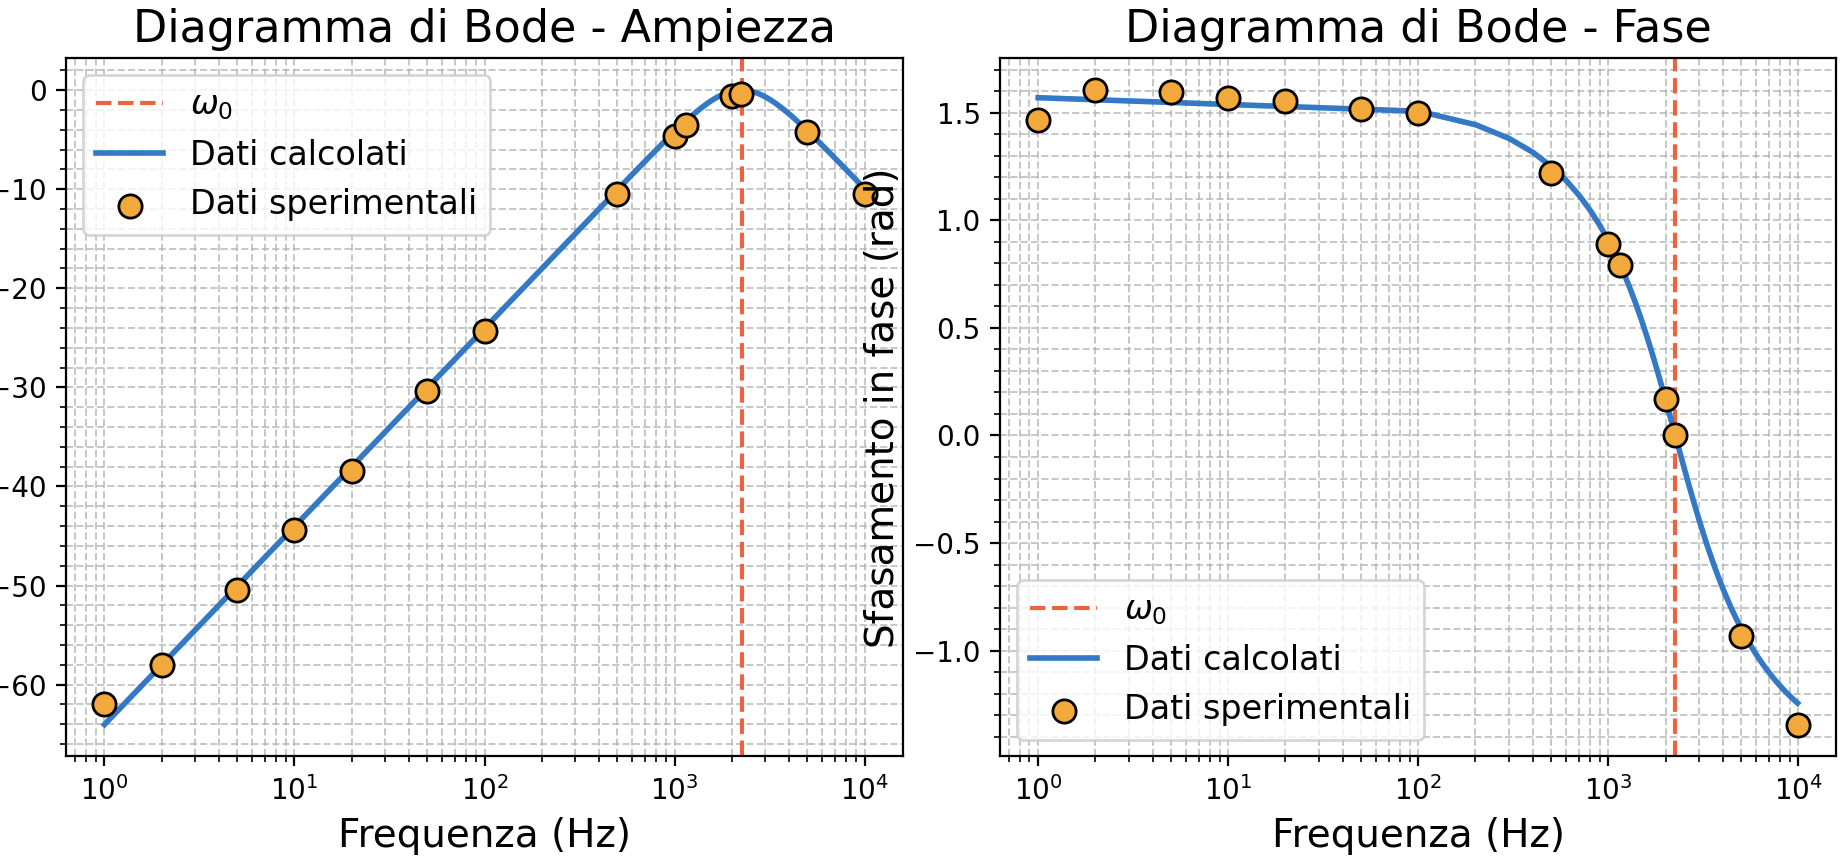
\includegraphics[width=0.6\linewidth]{bode1.png}
    \caption{Diagrammi di bode}
    \label{fig:enter-label}
\end{figure}
\begin{figure}[ht]
\centering
\begin{minipage}{0.5\textwidth}
\centering
\vspace{0pt}
    \centering
    \begin{tabular}{c|c|c|c}
        f & $\Delta$ & A_{ing} & A_{usc}\\
        \hline
        1Hz & 84\degree & 5V & 4mV \\
        \hline
        1,15KHz & 45,3\degree & 5V & 3,34V \\
        \hline
        2Hz & 92\degree & 5V & 6,25mV\\
        \hline
        4,5V & 47\degree & 5V & 3,38V \\
        \hline
        5Hz & 91,4\degree & 5V & 15,73mV \\
        \hline
        10Hz & 89,8\degree & 5V & 30,4mV \\
        \hline
        20Hz & 89\degree & 5V & 60,55mV \\
        \hline
        50Hz & 87\degree & 5V & 152mv \\
        \hline
        100Hz & 86\degree & 5V & 304,2mV \\
        \hline
        200Hz & 81\degree & 5V & 602,5mV \\
        \hline
        500Hz & 70\degree & 5V & 1,5V \\
        \hline
        1KHz & 51\degree & 5V & 2,93V \\
        \hline
        2KHz & 9,8\degree & 5V & 4,69V \\
        \hline
        2,25Khz & 0\degree & 5V & 4,77V \\
        \hline
        5Khz & -53,4\degree & 5V & 3,07V \\
        \hline
        10Khz & -77\degree & 5V & 1,5V \\
        \hline
        50KHz & - & 5V & - \\
    \end{tabular}
    \caption{RLC con resistenza 10k\ohm}
    \label{tab:my_label}
\label{fig:my_label}
\end{minipage}%
\begin{minipage}{0.5\textwidth}
\centering
\vspace{0pt}

Oltre a queste 13 misure, vengono
considerate altre tre frequenze: i due valori corrispondente ad un guadagno di -3 dB rispetto al suo massimo
e la frequenza di risonanza. Le prime sono state ottenute calcolando il guadagno a -3 dB, ottenuto
considerando il valore massimo di ampiezza del segnale di uscita misurato ai capi del resistore (4.77 V) diviso
la radice di 2:

$$A_{\epsilon dB} = \dfrac{A_{max}}{\sqrt{2}}=\dfrac{4,77V}{\sqrt{2}}=3,37V$$

Successivamente, si regola la frequenza dal generatore di segnali fino a quando non si ottiene un valore di
tensione paragonabile, in questo caso f1 = 1.15 kHz e f2 = 4.5 kHz.
Per quanto riguarda la frequenza di risonanza, essa è stata ricavata considerando prima il valore della
pulsazione in questione e poi dividendo per 2$\pi$:

$$\omega_0=\dfrac{1}{\sqrt{LC}}=14142\dfrac{rad}{s}$$
$$f_0=\dfrac{\omega_o}{2\pi}=2.25kHz$$

Per misurare l’ampiezza e lo sfasamento sull’oscilloscopio sono stati utilizzati gli appositi cursori, variando
opportunamente la scala dei tempi e dell’ampiezza.

 \end{minipage}
\end{figure}

I diagrammi di Bode (Figura 1) sono stati realizzati utilizzando i dati raccolti in laboratorio (Figura 2), facendo
attenzione allo sfasamento tra i due segnali ed effettuando la seguente conversione:
\begin{center}
    

$\Delta\O[rad]=\dfrac{\Delta t}{T}\cdot 2\pi$
\end{center}
Come è possibile notare, i risultati ottenuti sono coerenti con il comportamento passa-banda del circuito,
secondo il quale si ha un guadagno massimo( G = $\dfrac{A_{out}}{A_{in}}$) in corrispondenza della frequenza di risonanza,
mentre il segnale di uscita viene particolarmente attenuato a frequenze maggiori rispetto a 10 $f_0$ e inferiori rispetto a 0.1 $f_0$.

Utilizzando un valore di R pari a 10 k$\ohm$, le misure sono state effettuate variando il valore di frequenza del
segnale in ingresso da un minimo di 1 Hz a un massimo di 10 kHz.

\subsection{R= 1k$\ohm$}


\begin{figure}[H] % Usa H per mantenere la posizione della figura
    \centering
    \begin{minipage}[t]{0.5\textwidth} % Allineamento in alto
        \centering
        \vspace{0pt} % Per evitare spazi verticali aggiuntivi
        \begin{tabular}{c|c|c|c}
            f & $\Delta$ & A_{ing} & A_{usc} \\
            \hline
            1Hz & - & 5V & - \\
            \hline
            2Hz & - & 5V & - \\
            \hline
            2,03Hz & 45\degree & 5V & 2,4V \\
            \hline
            2,48Hz & 46\degree & 5V & 2,37V \\
            \hline
            5Hz & - & 5V & - \\
            \hline
            10Hz & 88\degree & 5V & 3,3mV \\
            \hline
            20Hz & 89\degree & 5V & 6,3mV \\
            \hline
            50Hz & 90\degree & 5V & 15,3mv \\
            \hline
            100Hz & 89\degree & 5V & 36,6mV \\
            \hline
            200Hz & 88\degree & 5V & 61mV \\
            \hline
            500Hz & 86,7\degree & 5V & 161mV \\
            \hline
            1KHz & 83\degree & 5V & 373mV \\
            \hline
            2KHz & 49,7\degree & 5V & 2,23V \\
            \hline
            5Khz & -85\degree & 5V & 383mV \\
            \hline
            10Khz & -88,6\degree & 5V & 155mV \\
            \hline
            50KHz & - & 5V & - \\
        \end{tabular}
        \caption{RLC con resistenza 1k$\ohm$}
        \label{tab:my_label}
    \end{minipage}%
    \begin{minipage}[t]{0.5\textwidth} % Allineamento in alto
        \centering
        \vspace{0pt} % Per evitare spazi verticali aggiuntivi
        In questo caso vengono ripetute le misure precedenti modificando il valore di R, andando perciò a variare il
        valore di tensione massima e di conseguenza le frequenze corrispondenti ad un valore di ampiezza inferiore
        di 3 dB rispetto a quello massimo, mentre la frequenza di risonanza rimane invariata in quanto i valori di
        capacità e induttanza sono invariati. Le misure a 1 e 2 Hz non sono state effettuate in quando il segnale di
        uscita in quel punto era molto attenuato e non era quindi osservabile all’oscilloscopio.

        $$A_{3dB}=\dfrac{3.37V}{\sqrt{2}}=2.38V$$
    \end{minipage}
\end{figure}

\begin{figure}[H]
    \centering
    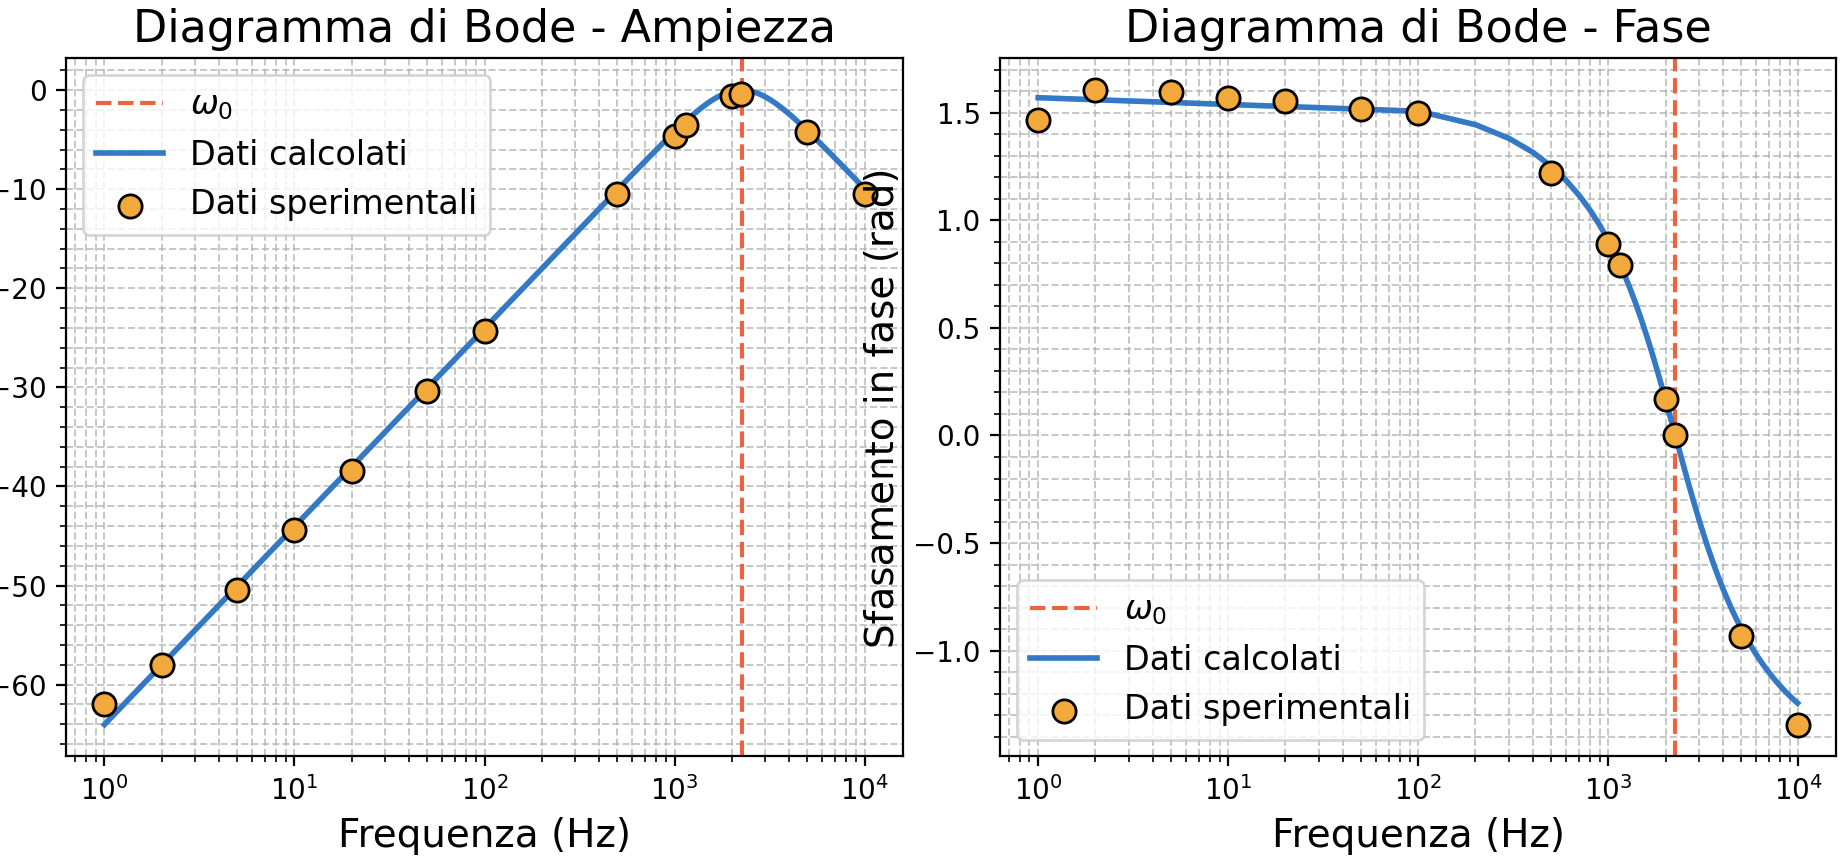
\includegraphics[width=0.6\linewidth]{bode2.png}
    \caption{Diagrammi di Bode}
    \label{fig:enter-label}
\end{figure}

Rispetto al caso precedente si nota come i valori di tensione misurati non rispecchiano perfettamente quelli
attesi, in particolar modo il valore massimo del segnale in uscita (3.37 V) è decisamente inferiore rispetto a
quello misurato con R = 10 k$\omega$ (4.77 V), e di conseguenza anche i valori relativi allo sfasamento. Ciò è causato
dal fatto che, avendo in questo caso un valore di resistenza più basso, esso è paragonabile al valore della
resistenza parassita presente in serie all’induttore a causa del suo comportamento reale:

\begin{figure}[!ht]
\centering %faccio un pane e nutella e torno %tranquillo amio <- cimelio storico
\resizebox{0.35\textwidth}{!}{%
\begin{circuitikz}
\tikzstyle{every node}=[font=\large]
\draw (8.75,14.75) to[C] (7.5,14.75);
\draw (11.25,14.75) to[R] (11.25,12.25);
\draw (11.25,14.75) to[short, -o] (12.5,14.75) ;
\draw (11.25,12.25) to[short, -o] (12.5,12.25) ;
\draw (11.25,12.25) to (11.25,12) node[ground]{};
\draw (7.5,12.25) to[short] (11.25,12.25);
\draw (7.5,12.25) to[sinusoidal voltage source, sources/symbol/rotate=auto] (7.5,14.75);
\draw (8.75,14.75) to[L ] (10,14.75);
\node [font=\large] at (12,14.75) {};
\draw (10,14.75) to[R] (11.25,14.75);
\node [font=\medium] at (7,13.75) {+};
\node [font=\medium] at (7,13.25) {-};
\node [font=\large] at (6.25,13.5) {$V_{in}(t)$};
\node [font=\large] at (8.15,15.4) {C};
\node [font=\large] at (9.35,15.25) {L};
\node [font=\large] at (10.7,15.25) {Rl};
\node [font=\large] at (10.5,13.5) {R};
\node [font=\large] at (13,13.5) {$V_{out}(t)$};
\node [font=\large] at (13,14.75) {+};
\node [font=\large] at (13,12.25) {-};
\end{circuitikz}
}%
\label{fig:my_label}
\end{figure}


Per stimare il suo valore, si considera un guadagno unitario del circuito ponendo a 0 i valori di capacità e di induttanza in modo da ottenere come unico elemento la serie tra il resistore R e la resistenza parassita Rl. Così facendo è possibile trovare il valore di tensione ai capi di Rl attraverso la legge di Kirchhoff delle maglie e successivamente la resistenza mediante la legge di Ohm (Vin = 5V, Vout = 3.37 V):

$$V_{Rl} = V_\text{in}-V_\text{out}=(5-3.37)V=1.63V$$

$$I=\frac{V_\text{out}}{R}=3.37mA$$

$$Rl = \frac{V_\text{Rl}}{I}=484\ohm$$

In questa esperienza dunque è stato appreso il concetto di resistenza parassita, che oltre a caratterizzare strumenti come oscilloscopi e multimetri, è caratteristica di qualsiasi oggetto presente nella realtà in quanto essi non rispettano le caratteristiche ideali secondo le quali solo i resistori offrono un valore di resistenza nel circuito.

\section{Esercizio 2}
Il secondo esercizio richiedeva di verificare il funzionamento del circuito RLC utilizzando come ingresso una forma d'onda quadra di frequenza 10Hz e tensione picco=picco di $V_\text{in}^\text{pp}=2.5V$, con offset $V_\text{in}^\text{of}=1.25V$, con varie combinazioni di R, L e C.

La risposta del circuito dipende dalla frequenza naturale del sistema, ossia la frequenza alla quale il circuito tenderebbe a oscillare se fosse lasciato libero, senza influenze esterne. Questa frequenza dipende dai valori di LL (induttore) e CC (condensatore) secondo la relazione:

$$f_0=\frac{1}{(2\pi\sqrt{LC})}$$

A questa frequenza, l’energia si scambia tra l’induttore (energia magnetica) e il condensatore (energia elettrica). Il valore di $R$, invece, introduce uno smorzamento che influisce sull’ampiezza delle oscillazioni nel tempo e modifica leggermente la frequenza effettiva delle oscillazioni, chiamata frequenza di oscillazione smorzata ($f_d$).
Il comportamento del circuito varia quindi come segue:
\begin{itemize}
    \item \textbf{Per valori crescenti di $L$}: un induttore più grande rallenta gli scambi energetici, riducendo la frequenza naturale $f_0$. Questo rende il circuito più lento a rispondere, con oscillazioni che avvengono a frequenze più basse.
     \item \textbf{Per valori crescenti di $C$}: un condensatore più grande consente di accumulare più carica, riducendo anch’esso la frequenza naturale $f_0$. Un CC elevato rende il circuito più dominato dalla reattanza capacitiva.
     \item \textbf{Per valori crescenti di $R$}: il valore della resistenza determina il grado di smorzamento del sistema. Se $R$ è basso, il circuito risponde in modo oscillatorio (regime sotto-smorzato), con oscillazioni persistenti ma a poco a poco attenuate. Al contrario, se $R$ è alto, il circuito diventa sovra-smorzato e la risposta non mostra oscillazioni ma solo un lento ritorno all’equilibrio.\\
     In generale, il circuito RLC serie può essere visto come un sistema in grado di oscillare con caratteristiche determinate da $L$ e $C$, mentre $R$ controlla l’attenuazione e la durata delle oscillazioni. Quando la resistenza è moderata, il circuito è \textbf{sotto-smorzato}, e le oscillazioni si verificano a una certa pulsazione $\omega_d$. 
     La frequenza smorzata $f_d=\omega_d/(2\pi)$ è leggermente inferiore a quella naturale $f_0$, ma per valori di $R$ non troppo elevati, questa differenza è trascurabile.
\end{itemize}
\label{fig:my_label}
\end{figure}

\begin{figure}[h]
    \centering
    \begin{minipage}[t]{0.33\textwidth} % Prima immagine
        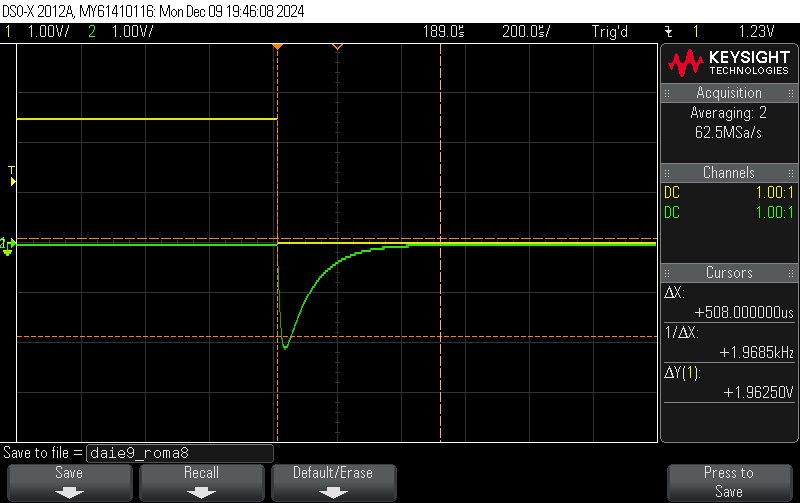
\includegraphics[width=0.9\linewidth]{dajeroma1.jpeg}
        \captionsetup{justification=raggedright, singlelinecheck=false, labelformat=empty}
        \caption{$R=10k\ohm, L=500mH, C=1nF$}
        \label{fig:img1}
    \end{minipage}%
    \hfill % Spaziatura uniforme tra le minipage
    \begin{minipage}[t]{0.33\textwidth} % Seconda immagine
        \centering
        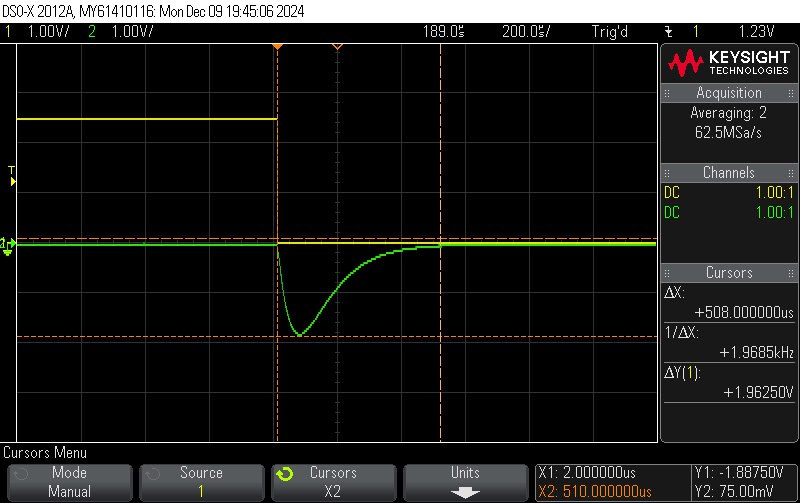
\includegraphics[width=0.9\linewidth]{dajeroma2.jpeg}
        \captionsetup{justification=raggedright, singlelinecheck=false, labelformat=empty}
        \caption{$R=10k\ohm, L=500mH, C=10nF$}
        \label{fig:img2}
    \end{minipage}%
    \hfill % Spaziatura uniforme tra le minipage
    \begin{minipage}[t]{0.33\textwidth} % Terza immagine
        \centering
        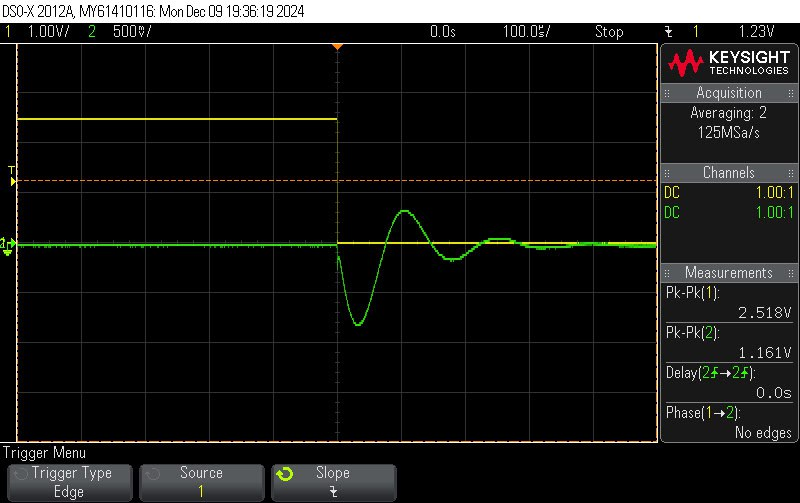
\includegraphics[width=0.9\linewidth]{dajeroma3.jpeg}
        \captionsetup{justification=raggedright, singlelinecheck=false, labelformat=empty}
        \caption{$R=10k\ohm, L=100mH, C=10nF$}
        \label{fig:img3}
    \end{minipage}
\end{figure}

Per il calcolo della frequenza di oscillazione nel primo caso si considera il periodo del segnale in questione, ottenuto spostando opportunamente gli appositi cursori dell’oscilloscopio, infine da esso si ricava il rispettivo valore di frequenza: 

$$T=0.143ms \hspace{30} f=\frac{1}{T}=7kHz$$

Successivamente, si confronta il valore di frequenza ottenuto sperimentalmente con quello ottenuto mediante le formule viste in precedenza e si nota come i due risultati coincidono:

$$\omega_0=\frac{1}{\sqrt{LC}}=44721\hpsace{30} f_0=\frac{\omega_0}{2\pi}=7.12kHz$$

In questa seconda esperienza è stato visto come, mettendo in ingresso un segnale ad onda quadra, il valore di uscita cambia variando resistenza, capacità e induttanza all’interno del circuito. In particolare, nel caso sotto-smorzato l’uscita è di tipo sinusoidale, mentre nel caso criticamente smorzato è di tipo esponenziale.

%ci avevo provato anche io

%eh ma sono troppo swaggg <- <3
%ho aggiunto una foto assolutamente essenziale
%odio i froci



%ez
%fortissimo

%boh io qua sinceramente non ho idea
%ma non ho capito, che sta da aggiungere? ciao mirko
%eh tipo tutto il punto 2.2 ma non so
%idk anche perche' abbiamo poco tempo
%amore mio, sono mirko.<-(smash) devo fare la relazione a mattia. cosa devo fare?
%non lo so manco io
%ti raidiamo casa, lol (penso stiano scherzando, ma te lo dico per il meme)
%a bo io sono qua

%dio negro, mattia non è molto utile. Non capisco che merda deve fare dio divoratore di peni persiani (dio stramaleddetto negro, non so come scrivere)

%la mia nuova bestemmia preferita e' dio orso che mangia la madonna salmonata


%ok dopo un aneurisma cerebrale credo di aver fatto dio mastrolindo
\label{fig:my_label}
\end{figure}
\end{document}